\documentclass{article}
\usepackage{amsmath}
\usepackage{amsfonts}
\usepackage{amssymb}
\usepackage[inline]{enumitem}
\usepackage[a4paper,margin=1in]{geometry}
\usepackage[normalem]{ulem}
\usepackage{graphicx}
\usepackage{tasks}
\settasks{label=(\alph*), label-offset=0.4em, label-width=1.5em}

\usepackage{fancyhdr}
\fancyhf{}
\setlength{\headheight}{36pt}
\renewcommand{\headrulewidth}{0pt}
\thispagestyle{fancy}
\lhead{Calculus Exercise}
\chead{Week 8 (4.5, 4.7, 4.9)}
\rhead{\underline{ID:\hspace{7.4em}} \\ \vspace{0.2cm} \underline{Name:\hspace{6em}}}
\cfoot{\thepage}

\begin{document}
\begin{enumerate}
\item[4.5.11]
    Sketch the curve
    \[
        y = \frac{x-x^{2}}{2 - 3x + x^{2}}
    \]

\vspace{6cm}

\item[4.5.37]
    Sketch the curve
    \[
        y = \sin (x) + \sqrt{3} \cos (x),\ -2 \pi \leqslant x \leqslant  2 \pi
    \]

\vspace{6cm}

\item[4.5.54]
    Sketch the curve
    \[
        y = \tan^{-1} \left(\frac{x-1}{x+1}\right)
    \]

\newpage

\item[4.5.56]
    The graph of a function $f$ is shown. (The dashed lines indicate
    horizontal asymptotes.) Find each of the following for the given
    function $g(x) = \sqrt[3]{f(x)}$.

    \begin{enumerate}
        \item The domains of $g$ and $g'$
        \item The critical numbers of $g$
        \item The approximate value of $g'(6)$
        \item All vertical and horizontal asymptotes of $g$
    \end{enumerate}

    \begin{center}
        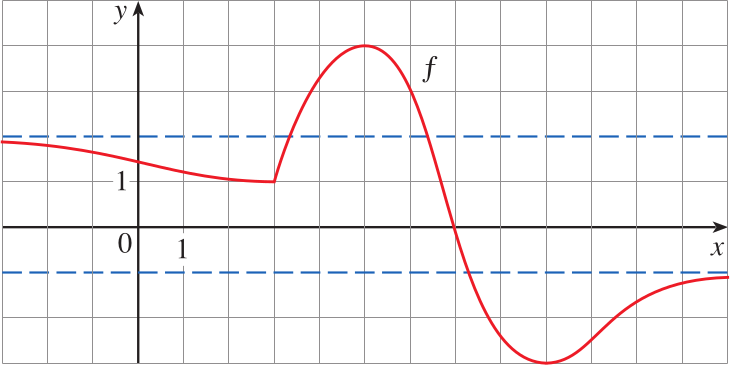
\includegraphics[width=8cm]{./png/4.5.56.png}
    \end{center}

\vspace{7cm}

\item[4.5.75]
    Show that the curve $y = x - \tan^{-1} (x) $ has two slant asymptotes:
    $y = x + \frac{\pi}{2}$ and $y = x - \frac{\pi}{2}$. Use this fact to help
    sketch the curve.

\newpage

\item[4.7.47]
    A cone-shaped drinking cup is made from a circular piece of paper of
    radius $R$ by cutting out a sector and joining the edges $CA$ and $CB$.
    Find the maximum capacity of such a cup.

    \begin{center}
        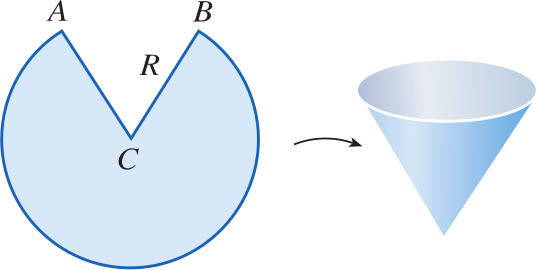
\includegraphics[width=5cm]{./png/4.7.47.png}
    \end{center}

\vspace{6cm}


\item[4.7.57]
    An oil refinery is located on the north bank of a straight river that is 2
    km wide. A pipeline is to be constructed from the refinery to storage tanks
    located on the south bank of the river 6 km east of the refinery. The cost
    of laying pipe is \$400,000/km over land to a point $P$ on the north bank
    and \$800,000/km under the river to the tanks. To minimize the cost of the
    pipeline, where should $P$ be located?

\newpage

\item[4.7.77]
    Let $v_1$ be the velocity of light in air and $v_2$ the velocity of light
    in water. According to Fermat's Principle, a ray of light will travel from
    a point $A$ in the air to a point $B$ in the water by a path $ACB$ that
    minimizes the time taken. Show that
    \[
        \frac{\sin ( \theta_{1} )}{\sin ( \theta_{2} )} = \frac{v_1}{v_2}
    \]
    where $\theta_{1}$ (the angle of incidence) and $ \theta_{2}$ (the angle of
    refraction) are as shown. This equation is known as Snell's Law.

    \begin{center}
        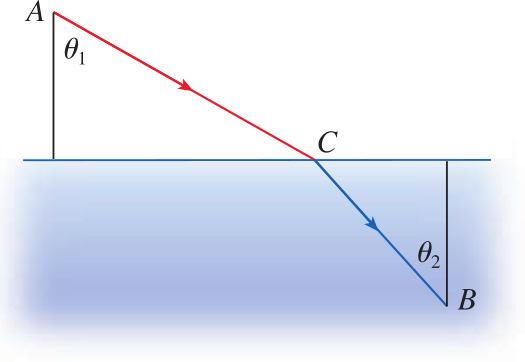
\includegraphics[width=5cm]{./png/4.7.77.png}
    \end{center}

\vspace{6cm}

\item[4.7.83]
    Where should the point $P$ be chosen on the line segment $AB$ so as to
    maximize the angle $ \theta $?

    \begin{center}
        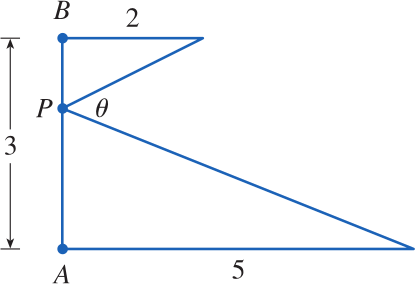
\includegraphics[width=5cm]{./png/4.7.83.png}
    \end{center}

\newpage

\item[4.7.88]
    Two light sources of identical strength are placed 10 m apart.
    An object is to be placed at a point $P$ on a line $l$, parallel to
    the line joining the light sources and at a distance $d$ meters
    from it (see the figure). We want to locate $P$ on $l$ so that the
    intensity of illumination is minimized. We need to use the fact
    that the intensity of illumination for a single source is directly
    proportional to the strength of the source and inversely proportional
    to the square of the distance from the source.

    \begin{enumerate}
        \item Find an expression for the intensity $I(x)$ at the point $P$.
        \item If $d = 5$m, use graphs of $I(x)$ and $I'(x)$ to show that
            the intensity is minimized when $x=5$m, that is, when $P$ is
            at the midpoint of $l$.
        \item If $d = 10$m, show that the intensity (perhaps surprisingly)
            is \textit{not} minimized at the midpoint.
        \item Somewhere between $d=5$ m and $d=10$ m there is a transitional
            value of $d$ at which the point of minimal illumination abruptly
            changes. Estimate this value of $d$ by graphical methods.
            Then find the exact value of $d$.
    \end{enumerate}

    \begin{center}
        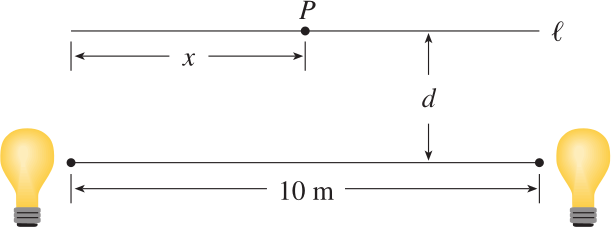
\includegraphics[width=7cm]{./png/4.7.88.png}
    \end{center}

\newpage

\item[4.9.4]
    Find an antiderivative of the function
    \[
        f(x) = \frac{1}{x}
    \]

\vspace{3cm}

\item[4.9.12]
    Find the most general antiderivative of the function
    \[
        f(x) = 3x^{0.8} + x^{-2.5}
    \]

\vspace{6cm}

\item[4.9.24]
    Find the most general antiderivative of the function
    \[
        f(x) = 2 \cos (x) - \frac{3}{\sqrt{1-x^{2}}}
    \]

\newpage

\item[4.9.42]
    Find $f$
    \[
        f'(x) = \frac{x+1}{\sqrt{x}},\ f(1) = 5
    \]

\vspace{6cm}

\item[4.9.52]
    Find $f$
    \[
        f''(x) = \sqrt[3]{x} - \cos (x),\ f(0) = f(1) = 2
    \]
\end{enumerate}
\end{document}
